\documentclass[12pt]{article}
\usepackage[english]{babel}
\usepackage{natbib}
\usepackage{url}
\usepackage[utf8x]{inputenc}
\usepackage{amsmath}
\usepackage{graphicx}
\graphicspath{{images/}}
\usepackage{parskip}
\usepackage{fancyhdr}
\usepackage{vmargin}
\setmarginsrb{3 cm}{2.5 cm}{3 cm}{2.5 cm}{1 cm}{1.5 cm}{1 cm}{1.5 cm}

\title{19. Cálculo de la temperatura de saturación}								% Title
\author{Santiago Sanz Wuhl}								% Author
\date{18 Dic 2018}											% Date

\makeatletter
\let\thetitle\@title
\let\theauthor\@author
\let\thedate\@date
\makeatother

\pagestyle{fancy}
\fancyhf{}
\rhead{\theauthor}
\lhead{\thetitle}
\cfoot{\thepage}

\begin{document}

%%%%%%%%%%%%%%%%%%%%%%%%%%%%%%%%%%%%%%%%%%%%%%%%%%%%%%%%%%%%%%%%%%%%%%%%%%%%%%%%%%%%%%%%%

\begin{titlepage}
	\centering
    \vspace*{0.5 cm}
    
\includegraphics[scale = 0.15]{logo.png}\\[1.0 cm]	% University Logo
    % University Name
	\textsc{\Large 1º Física}\\[0.5 cm]				% Course Code
	\rule{\linewidth}{0.2 mm} \\[0.4 cm]
	{ \huge \bfseries \thetitle}\\
	\rule{\linewidth}{0.2 mm} \\[1.5 cm]
	 \large Santiago Sanz Wuhl

	
\end{titlepage}

%%%%%%%%%%%%%%%%%%%%%%%%%%%%%%%%%%%%%%%%%%%%%%%%%%%%%%%%%%%%%%%%%%%%%%%%%%%%%%%%%%%%%%%%%

\tableofcontents
\pagebreak

%%%%%%%%%%%%%%%%%%%%%%%%%%%%%%%%%%%%%%%%%%%%%%%%%%%%%%%%%%%%%%%%%%%%%%%%%%%%%%%%%%%%%%%%%

\section{Fundamento Teórico}
    La temperatura a la cual cierto líquido hierve dependerá únicamente de la presión a la que esté sometido. A esta temperatura, de saturación,  se llega cuando la sustancia en fase líquida entra en equilibrio dinámico con la fase gaseosa de la misma. \\
 \begin{wrapfigure}{1}{5} %this figure will be at the right
    \centering
    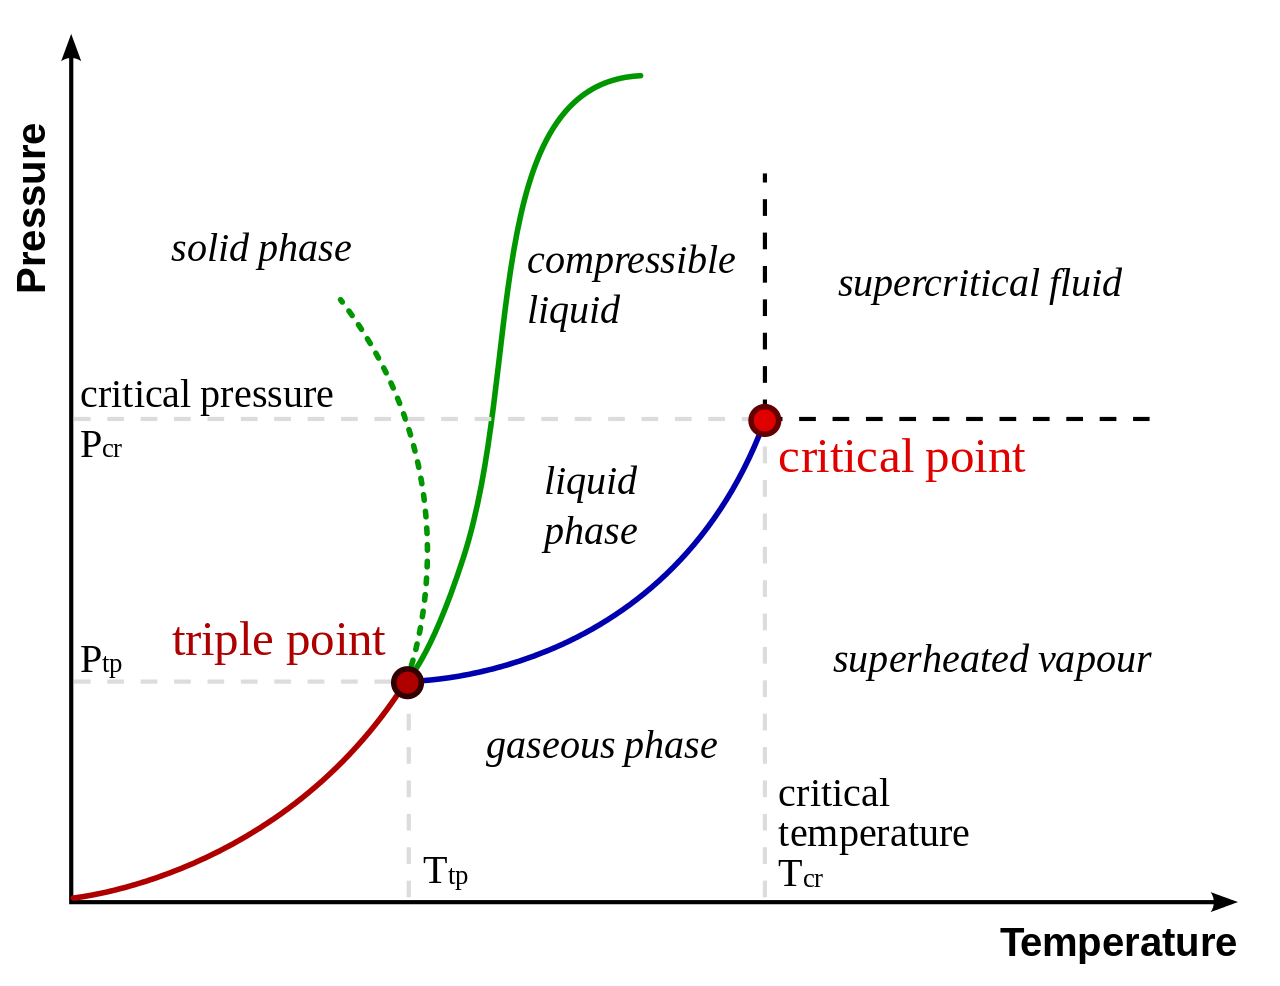
\includegraphics[scale = 0.2]{diagfase.png}
\end{wrapfigure}
    

A Table of Contents and a bibliography have also been implemented. To add entries to your bibliography, simply edit \texttt{biblist.bib} in the root folder and then use the \texttt{\textbackslash cite\{\ldots\}} command in \texttt{main.tex} \cite{bibtex}. The Table of Contents will be updated automatically.

I hope that you find this template both visually appealing and useful. \\

\hspace{1 cm}--- Linus

\newpage
\bibliographystyle{plain}
\bibliography{biblist}

\end{document}